\graphicspath{{chapters/software/}}


\chapter{CCA-Zoo: A collection of Regularized, Deep Learning-based, Kernel, and Probabilistic methods in a scikit-learn style framework}\label{ch:software}

% \epigraph{And that's really the essence of programming. By the time you've sorted out a complicated idea into little steps that even a stupid machine can deal with, you've learned something about it yourself.}{\textit{Douglas Adams}}
\section*{Preface}

This work was published in the Journal of Open Source Software \citep{chapman2021cca}.
I have been the lead developer of the \texttt{CCA-Zoo} package since its inception in 2020.
All of the methods we have described in this thesis are implemented in \texttt{CCA-Zoo} and are immediately available for use by the research community.

\section{Introduction}

The Python programming language has seen a surge in popularity in the machine learning community due to its versatility and extensive libraries.
However, when it comes to the domain of multiview learning, there is a noticeable void in the Python ecosystem.
Existing libraries, such as \texttt{scikit-learn}\cite{pedregosa2011scikit}, offer basic implementations for CCA and PLS, yet fall short of providing a comprehensive toolkit for multiview learning techniques.
This is particularly striking given the widespread recognition that the availability of quality software implementations often acts as a catalyst for the adoption of novel methodologies in the statistical learning community.

One glaring example of this trend is Sparse PLS. Despite its known limitations, Sparse PLS has effectively become the go-to method for sparse CCA applications, primarily due to its robust implementation in the R programming language.
The discrepancy between the availability of multiview learning tools in R and Python has not only hindered the diversification of methodologies but also impeded the community from leveraging the more recent advances in the field.

\section{Background}

The research community continues to show a heightened interest in multiview learning.
Traditionally, this field has been dominated by contributions from statistical learning researchers who predominantly used R and MATLAB for their work.
These platforms have been the birthplace of many state-of-the-art algorithms and methodologies, including Sparse PLS.

However, this posed a challenge for Python-oriented researchers and practitioners, leaving them with two less-than-ideal options: either port existing R or MATLAB code into Python, often a non-trivial task requiring domain expertise, or resort to using the limited set of methods available in native Python libraries like \texttt{scikit-learn}.
This fragmentation has, in effect, created barriers to entry and possibly slowed down the progress in applying multiview learning techniques in Python-based projects.

The \texttt{CCA-Zoo} package aims to bridge this divide by offering a broad range of multiview learning algorithms, creating a unified platform that fosters both academic research and practical applications in Python.

\section{Methods}

In this section, we describe the implementation of \texttt{CCA-Zoo} as depicted in Figure \ref{fig:cca-zoo-api} and the design decisions that were made during its development.
We highlight the package's optimization for use with high-dimensional biomedical data and elaborate on its compatibility with standard machine learning packages.

\subsection{API}

\begin{figure}[ht]
    \centering
    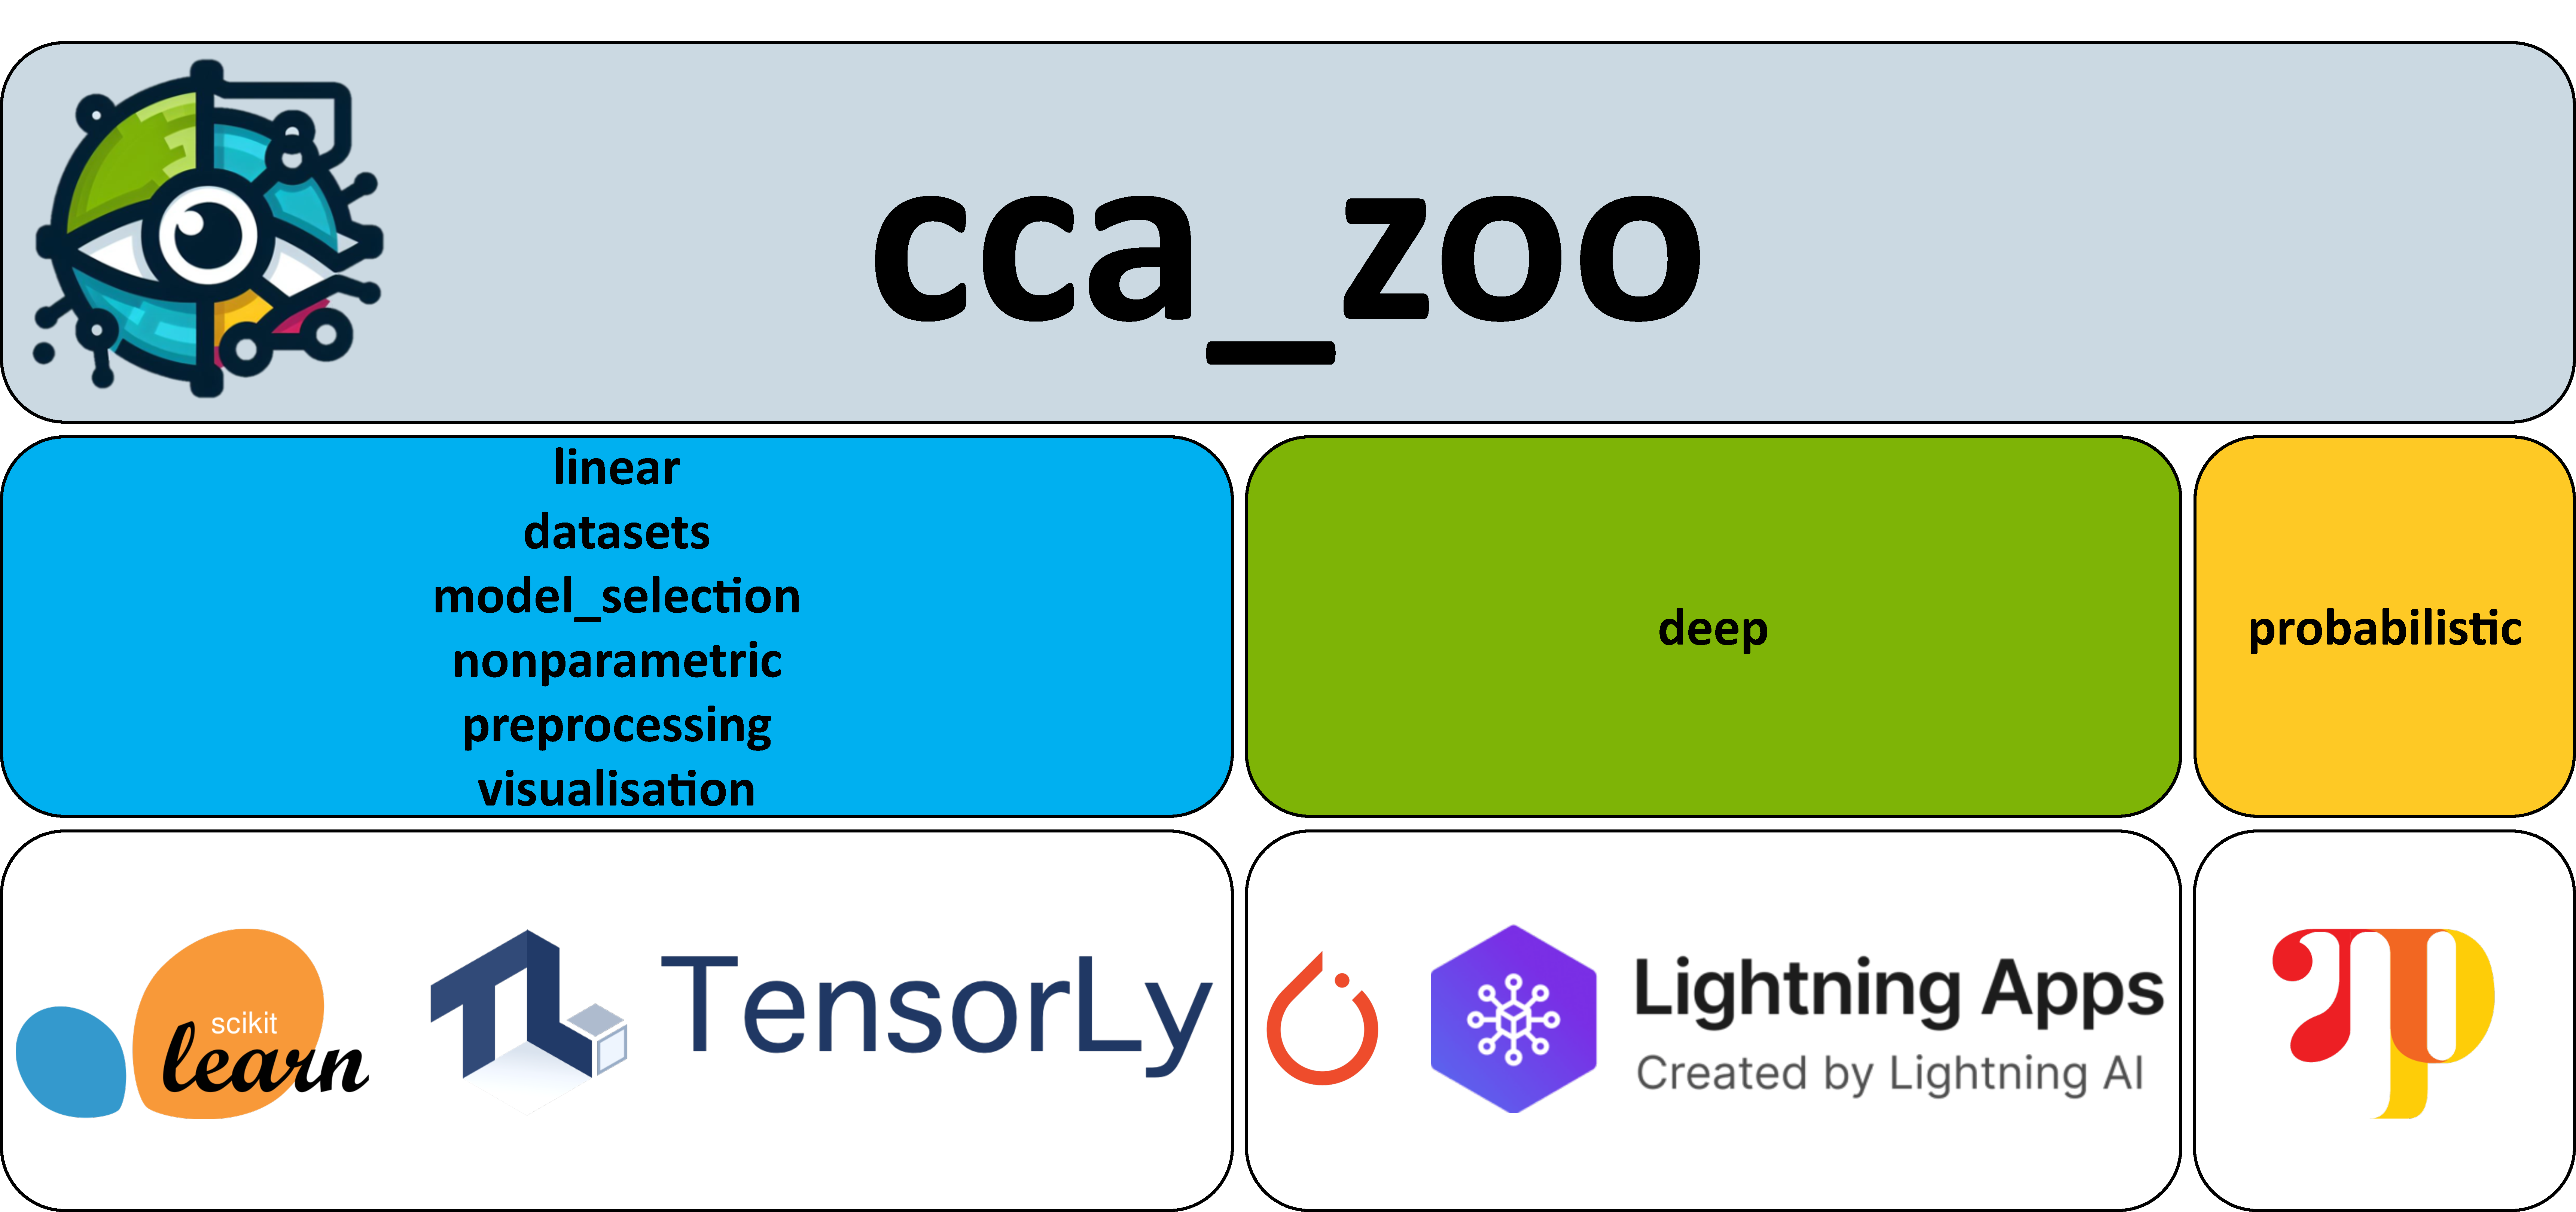
\includegraphics[width=0.8\textwidth]{figures/CCA_Zoo_map}
    \caption[The \texttt{CCA-Zoo} compatibility map]{The \texttt{CCA-Zoo} compatibility map showcases integration with various machine learning packages. The deep learning module is built upon \texttt{PyTorch} and \texttt{Lightning}, reflecting their status as industry standards for neural network implementations. The probabilistic module employs \texttt{NumPyro} for its Bayesian inference capabilities, enhancing the application of probabilistic approaches in CCA.}
    \label{fig:cca-zoo-api}
\end{figure}

The \texttt{scikit-learn} API is familiar to many machine learning practitioners and researchers, and is the de facto standard for machine learning in Python. \texttt{CCA-Zoo} has been designed to be consistent with the \texttt{scikit-learn} API, inheriting its user-friendly characteristics and ensuring compatibility with the \texttt{scikit-learn} ecosystem. Furthermore, the deep module within \texttt{CCA-Zoo} integrates \texttt{PyTorch} and \texttt{Lightning}, harnessing their powerful features for deep learning research and applications. The probabilistic module takes advantage of \texttt{NumPyro}, which offers advanced features for probabilistic programming and Bayesian methods, further extending the versatility and functionality of \texttt{CCA-Zoo}.


\subsection{Usage}

The \texttt{CCA-Zoo} package is a comprehensive toolkit that includes modules for datasets, preprocessing, model selection, various models (linear, deep, nonparametric, probabilistic), and visualization.
It is designed to plug seamlessly into \texttt{scikit-learn} pipelines, allowing users to select and utilize components as needed.
This design enhances the flexibility and applicability of multiview learning methods.

In this section, we will walk through the complete \texttt{CCA-Zoo} workflow, from data generation to model selection and evaluation.
We will highlight the package's design choices and its integration capabilities. Figure \ref{fig:cca-zoo-pipeline} illustrates the overall structure and flow of the \texttt{CCA-Zoo} pipeline, demonstrating its compatibility with the \texttt{scikit-learn} API and how it facilitates integration with existing machine learning workflows.

\begin{figure}[ht]
    \centering
    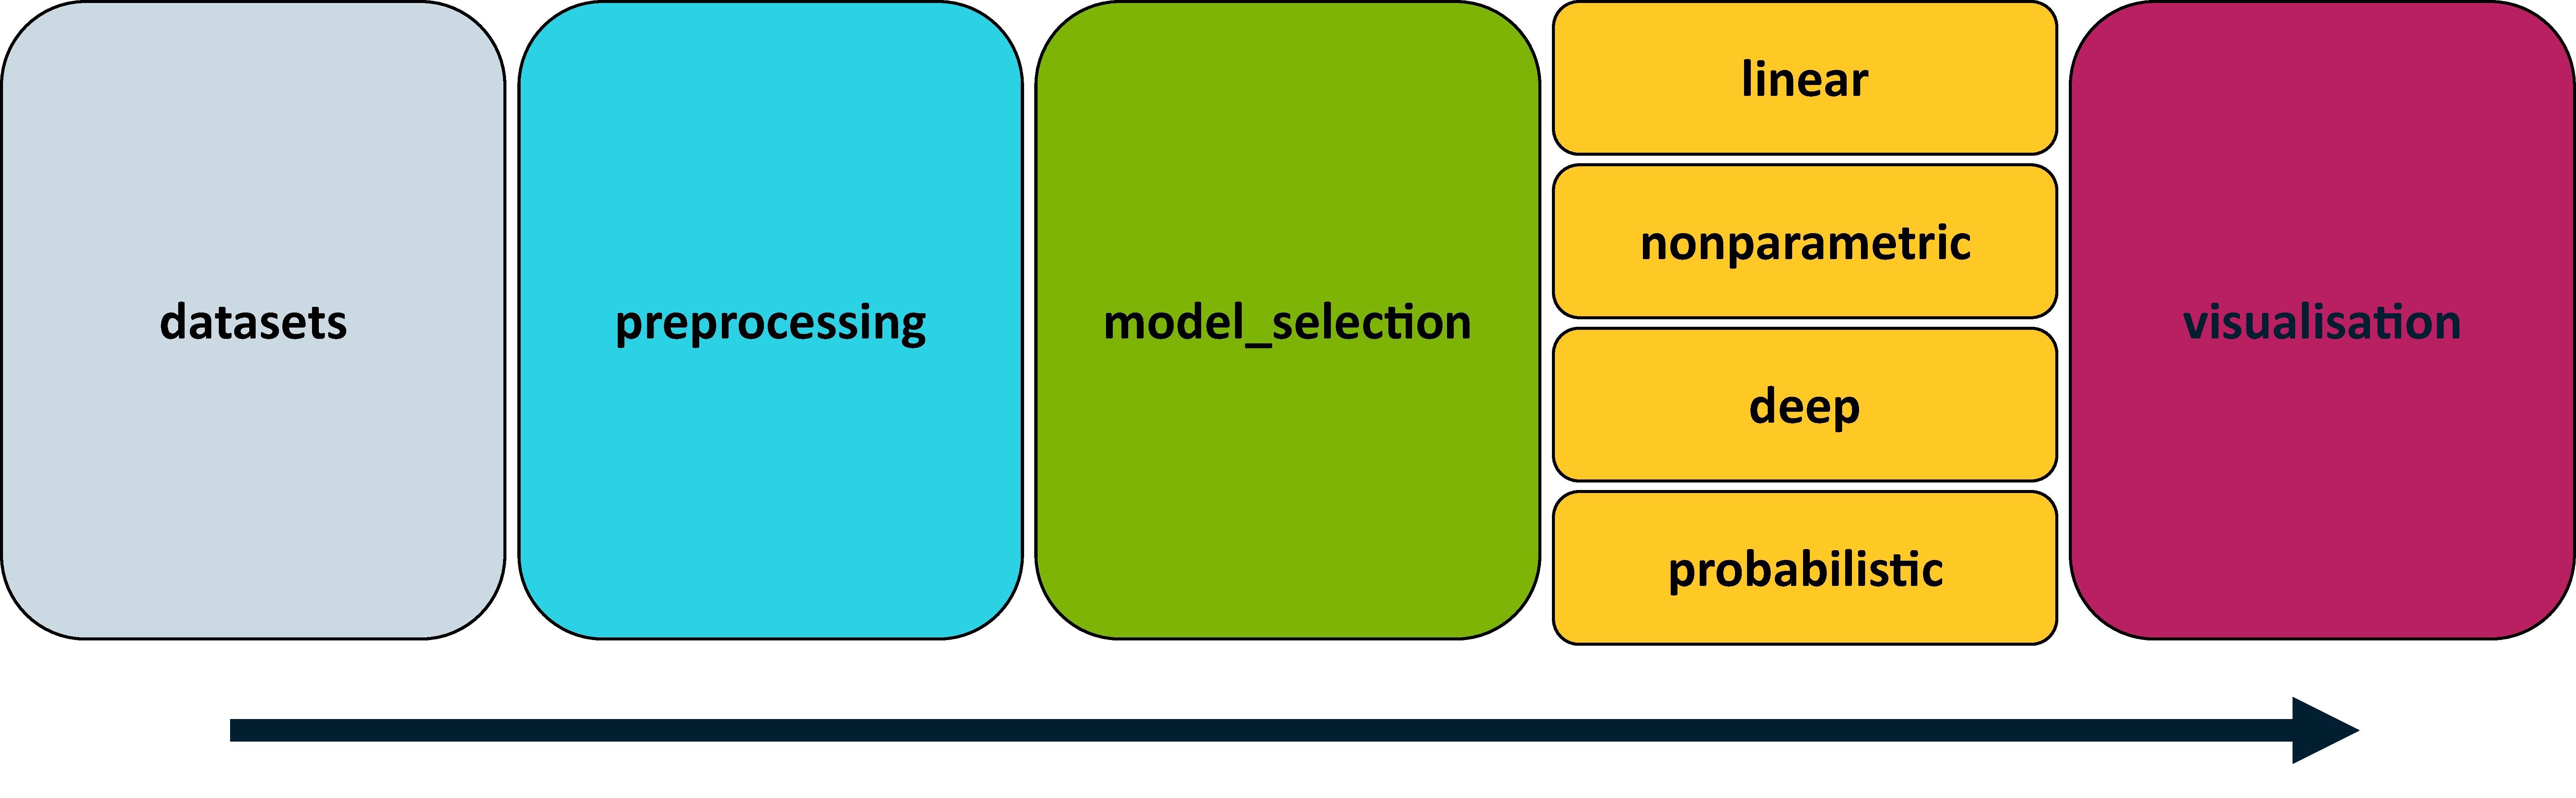
\includegraphics[width=0.8\textwidth]{figures/pipeline}
    \caption[The \texttt{CCA-Zoo} pipeline]{The \texttt{CCA-Zoo} pipeline. Designed for compatibility with the \texttt{scikit-learn} API, it facilitates integration with existing machine learning workflows.}\label{fig:cca-zoo-pipeline}
\end{figure}

The complete pipeline for \texttt{CCA-Zoo} is straightforward and user-friendly.
The following example demonstrates the implementation of a regularized CCA model with a ridge penalty, showcasing the practical application of the pipeline:

\begin{minted}{python}
    # Import required libraries
    import numpy as np
    from cca_zoo.datasets import LatentVariableData
    from cca_zoo.preprocessing import
    from cca_zoo.linear import rCCA
    from cca_zoo.model_selection import GridSearchCV
    from cca_zoo.visualisation import Di
    
    # Generate synthetic multiview data
    data = LatentVariableData(view_features=[10,10],latent_dims: int = 2)
    (X,Y) = data.sample(n_samples=100)

    # Define grid of potential regularization parameters
    c1 = [0.1, 0.3, 0.7, 0.9]
    c2 = [0.1, 0.3, 0.7, 0.9]
    param_grid = {'c': [c1, c2]}

    cv = 5  # Number of folds in cross-validation

    # Conduct grid search
    ridge = GridSearchCV(rCCA(latent_dimensions=2), param_grid=param_grid,
                        cv=cv, verbose=True, scoring=scorer).fit((train_view_1, train_view_2))
    # Get best model
    best_model = ridge.best_estimator_

    # Visualize


    \end{minted}

\subsection{Datasets}
\texttt{CCA-Zoo} provides a range of datasets for testing and benchmarking, which are outlined in Table \ref{tab:class_method_6}.
These datasets are designed to be compatible with the \texttt{scikit-learn} API, allowing users to easily integrate them into their workflows.
In particular, this module includes the LatentVariableData class which implements the explicit latent variable model and JointData which implements the implicit latent variable model described in Chapter \ref{ch:loadings}.
Additionally, \texttt{CCA-Zoo} includes a variety of real-world datasets, including the MNIST, CIFAR10, and Mfeat datasets, as well as the Breast Cancer dataset from the UCI repository which has been used extensively in the literature\cite{witten2009penalized}.

\begin{table}[ht]
    \centering
    \begin{tabular}{|c|c|}
        \hline
        Class Name & Method Name \\
        \hline
        LatentVariableData & Latent Variable Data \\
        JointData & Joint Data \\
        load\_breast\_data & Breast Cancer Data \\
        load\_split\_cifar10\_data & CIFAR10 Data \\
        load\_split\_mnist\_data & MNIST Data \\
        load\_mfeat\_data & Mfeat Data \\
        \hline
    \end{tabular}
    \caption{Class Names and Method Names}\label{tab:class_method_6}
\end{table}

\subsection{Model Selection Utilities}
For model selection and evaluation, \texttt{CCA-Zoo} includes various utilities as shown in Table \ref{tab:class_method_5}.
The existing \texttt{scikit-learn} API contains a number of methods for model selection, including GridSearchCV and RandomizedSearchCV as well as permutation tests and learning curves.
Unfortunately, these methods are not compatible with multiview learning methods, which have separate parameters for each view.
To address this issue, \texttt{CCA-Zoo} puts a thin wrapper around these methods, combining multiview parameter combinations so that they appear as single view models to \texttt{scikit-learn}, but splitting them back into their constituent views when fitting the model.
This means that \texttt{CCA-Zoo} benefits from the multiprocessor capabilities of \texttt{scikit-learn} as well as a standardized outputs including the \texttt{best\_estimator\_} attribute, model fit times, and a dictionary summarizing the results of the cross-validation.

\begin{table}[ht]
    \centering
    \begin{tabular}{|c|c|}
        \hline
        Class Name & Method Name \\
        \hline
        GridSearchCV & Grid Search Cross Validation \\
        RandomizedSearchCV & Randomized Search Cross Validation \\
        cross\_validate & Cross Validation \\
        learning\_curve & Learning Curve \\
        permutation\_test\_score & Permutation Test Score \\
        \hline
    \end{tabular}
    \caption{Class Names and Method Names}\label{tab:class_method_5}
\end{table}

\subsection{Linear}
In this section, we explore a variety of linear multiview learning methods available in \texttt{CCA-Zoo}, as detailed in Table \ref{tab:class_method}.


\begin{table}[ht]
    \centering
    \begin{tabular}{|c|c|}
        \hline
        Class Name & Method Name \\
        \hline
        MCCA & Multiview (Ridge) CCA\citep{rupnik2010multi} \\
        CCA & Canonical Correlation Analysis\citep{hotelling1992relations} \\
        rCCA & Ridge CCA\citep{vinod1976canonical} \\
        PLS & Partial Least Squares\cite{wold1975path} \\
        MPLS & Multiview Partial Least Squares \\
        GCCA & Generalized (Ridge) CCA\citep{carroll1968generalization, tenenhaus2011regularized} \\
        GRCCA & Group Ridge Regularized CCA\citep{tuzhilina2023canonical} \\
        PartialCCA & Partial CCA\citep{rotman2018bridging} \\
        PRCCA &  \citep{tuzhilina2023canonical}\\
        TCCA & Tensor CCA\citep{kim2007tensor} \\
        PCACCA & PCA-CCA\citep{mihali} \\
        SCCA\_IPLS & Sparse CCA using Iterative Lasso \\
        ElasticCCA & Elastic CCA using FRALS \\
        PLS\_ALS & PLS using Alternating Least Squares \\
        SPLS & Sparse PLS \\
        SCCA\_Parkhomenko & Penalized CCA \\
        SCCA\_Span & Sparse CCA using Span Bound \\
        CCA\_EY & CCA by Eckart-Young \\
        PLS\_EY & PLS by Eckart-Young \\
        CCA\_GHA & CCA using Generalized Hebbian Algorithm \\
        CCA\_SVD & CCA using SVD \\
        PLSStochasticPower & PLS using Stochastic Power Method \\
        \hline
    \end{tabular}
    \caption{Class Names and Method Names}
    \label{tab:class_method}
\end{table}


\subsection{Deep}
Table \ref{tab:class_method_2} lists the deep learning methods implemented in \texttt{CCA-Zoo}, offering advanced capabilities for deep canonical correlation analysis and related techniques.

\begin{table}[ht]
    \centering
    \begin{tabular}{|c|c|}
        \hline
        Class Name & Method Name \\
        \hline
        DCCA & Deep CCA \\
        DCCA\_GHA & Deep CCA by Generalized Hebbian Algorithm \\
        DCCA\_SVD & Deep CCA by SVD \\
        DMCCA & Deep Multiview CCA \\
        DGCCA & Geep Generalised CCA \\
        DCCAE & Deep Canonically Correlated Autoencoders \\
        DCCA\_NOI & Deep CCA by nonlinear orthogonal iterations \\
        DCCA\_SDL & Deep CCA by stochastic decorrelation loss \\
        DVCCA & Deep Variaitional CCA \\
        BarlowTwins & Barlow Twins \\
        VICReg & VICReg \\
        DTCCA & Deep Tensor CCA \\
        DCCA\_EY & Deep CCA by Eckart-Young \\
        architectures & \\
        \hline
    \end{tabular}
    \caption{Class Names and Method Names}\label{tab:class_method_2}
\end{table}

\subsection{Probabilistic}
The probabilistic methods in \texttt{CCA-Zoo}, including variations of probabilistic CCA and PLS, are summarized in Table \ref{tab:class_method_3}.
While we have not explored these methods in detail in this thesis, they are included in \texttt{CCA-Zoo} for completeness and to facilitate future research.
Probabilistic methods for multiview learning are an active area of research, that is notably limited by computational constraints.
Existing publicly available implementations use the Expectation-Maximization algorithm, which is efficient for simple models but can be slow to converge.
By leveraging a GPU-enabled probabilistic programming language, \texttt{CCA-Zoo} can use stochastic variational inference to speed up the training process, or MCMC sampling to obtain more accurate estimates of the posterior distribution.

\begin{table}[ht]
    \centering
    \begin{tabular}{|c|c|}
        \hline
        Class Name & Method Name \\
        \hline
        PCCA & Probabilistic CCA \\
        PPLS & Probabilistic PLS \\
        \hline
    \end{tabular}
    \caption{Class Names and Method Names}\label{tab:class_method_3}
\end{table}

\subsection{Nonparametric}
Table \ref{tab:class_method_4} presents the nonparametric methods in \texttt{CCA-Zoo}, focusing on kernel-based techniques for multiview learning.


\begin{table}[ht]
    \centering
    \begin{tabular}{|c|c|}
        \hline
        Class Name & Method Name \\
        \hline
        KCCA & Kernel CCA \\
        KPLS & Kernel PLS \\
        \hline
    \end{tabular}
    \caption{Class Names and Method Names}\label{tab:class_method_4}
\end{table}

\subsection{Visualization}
\texttt{CCA-Zoo} also provides a range of visualization tools for multiview learning, which are outlined in Table \ref{tab:vis_method}.

\begin{table}[ht]
    \centering
    \begin{tabular}{|c|c|}
        \hline
        Class Name & Method Name \\
        \hline
        ExplainedVarianceDisplay & Explained Variance Display \\
        RepresentationScatterDisplay & Representation Scatter Display \\
        JointRepresentationScatterDisplay & Joint Representation Scatter Display \\
        SeparateRepresentationScatterDisplay & Separate Representation Scatter Display \\
        SeparateJointRepresentationDisplay & Separate Joint Representation Display \\
        PairRepresentationScatterDisplay & Pair Representation Scatter Display \\
        ExplainedCovarianceDisplay & Explained Covariance Display \\
        WeightHeatmapDisplay & Weight Heatmap Display \\
        CorrelationHeatmapDisplay & Correlation Heatmap Display \\
        CovarianceHeatmapDisplay & Covariance Heatmap Display \\
        \hline
    \end{tabular}
    \caption{Class Names and Method Names for Visualization in \texttt{CCA-Zoo}}\label{tab:vis_method}
\end{table}

\subsection{Code Availability}

The code for \texttt{CCA-Zoo} is available at.

\texttt{CCA-Zoo} has received 155 stars and 30 forks on GitHub, and has nearly 500 downloads per month on PyPI \footnote{https://pypistats.org/packages/cca-zoo}.

Documentation for \texttt{CCA-Zoo} is available at \footnote{https://cca-zoo.readthedocs.io/en/latest/}.
The documentation includes a user guide, API reference, and examples.

The package can be installed using \texttt{pip install cca-zoo} or \texttt{poetry add cca-zoo}.

\section{Benchmarking}

In this section, we compare the performance of \texttt{CCA-Zoo} against \texttt{scikit-learn}, focusing on the efficiency of the basic CCA and PLS methods.
We conducted experiments on synthetic datasets with varying dimensions to evaluate their average execution time.
The datasets consisted of random matrices with a varying number of dimensions: \(50\), \(100\), \(200\), \(400\), and \(800\).
Each matrix had \(100\) samples.
We set the latent dimensions for both CCA and PLS to \(10\).
For each dimension, the experiment was repeated \(10\) times to obtain reliable performance metrics.

\paragraph{Libraries Used:}
\begin{itemize}
    \item \texttt{CCA-Zoo} (version: 2.4.0)
    \item \texttt{Scikit-learn} (version: 1.3.0)
\end{itemize}

\subsection{Canonical Correlation Analysis:}
Figure~\ref{fig:cca_benchmark} presents the comparison between \texttt{CCA-Zoo} and \texttt{scikit-learn} for Canonical Correlation Analysis.
We observe that \texttt{CCA-Zoo} exhibits a competitive runtime profile when compared to \texttt{scikit-learn} across all dimensions.
This is because \texttt{CCA-Zoo} computes CCA in the principal component space, which is more efficient than the standard approach of computing the covariance matrices directly for high dimensional data.

\begin{figure}[h]
    \centering
    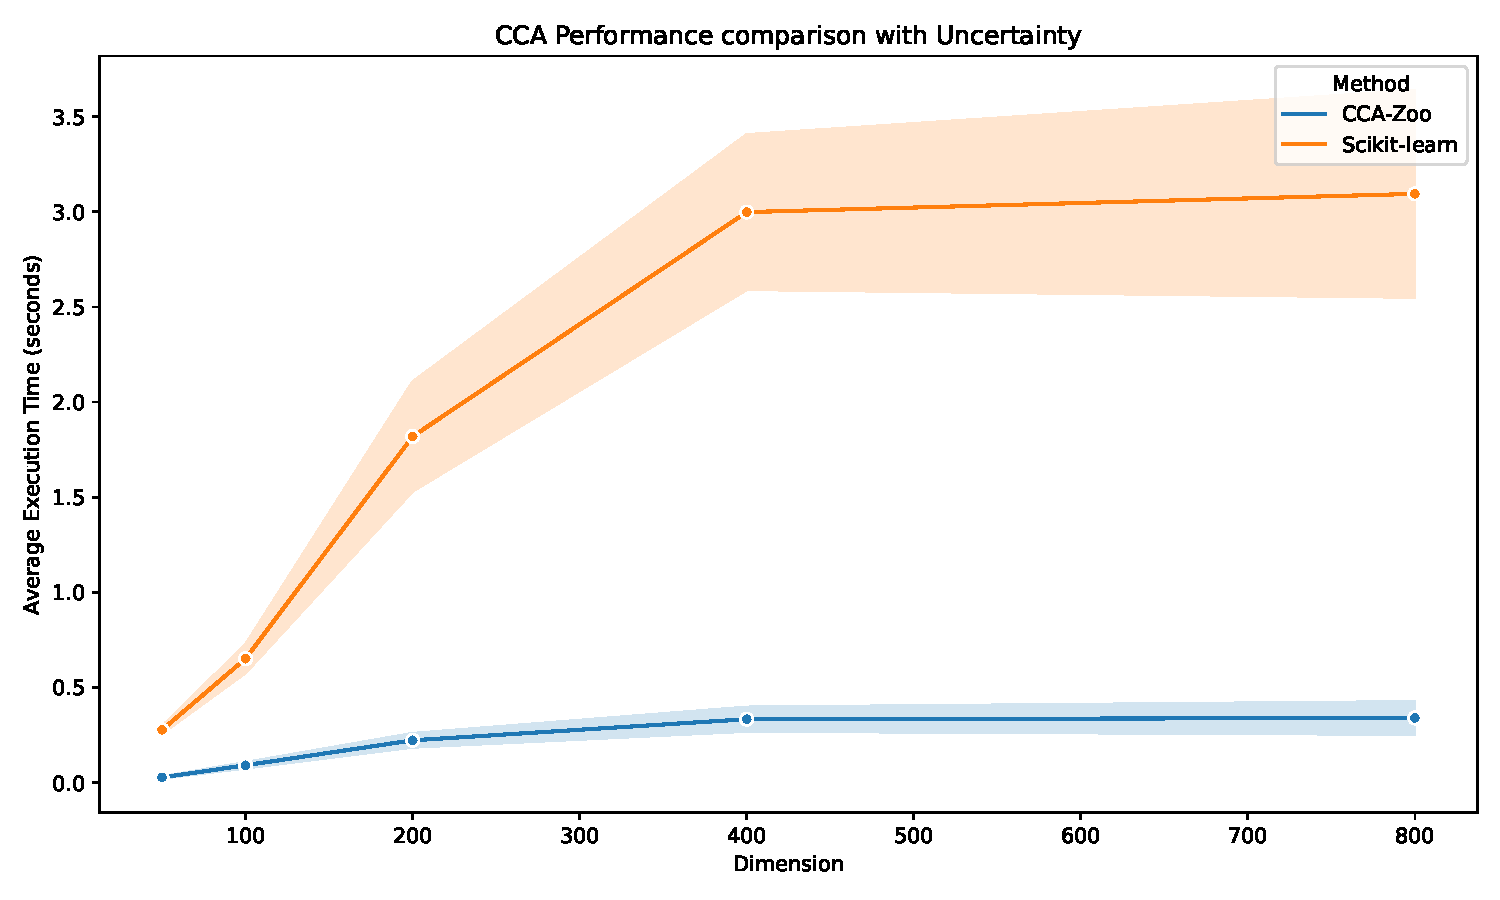
\includegraphics[width=0.9\textwidth]{figures/CCA_Speed_Benchmark}
    \caption{Performance comparison for CCA methods}
    \label{fig:cca_benchmark}
\end{figure}

\subsection{Partial Least Squares:}
The comparison for Partial Least Squares is shown in Figure \ref{fig:pls_benchmark}.
Like the CCA experiment, \texttt{CCA-Zoo} maintains a robust performance profile that is competitive with \texttt{scikit-learn}.

\begin{figure}[h]
    \centering
    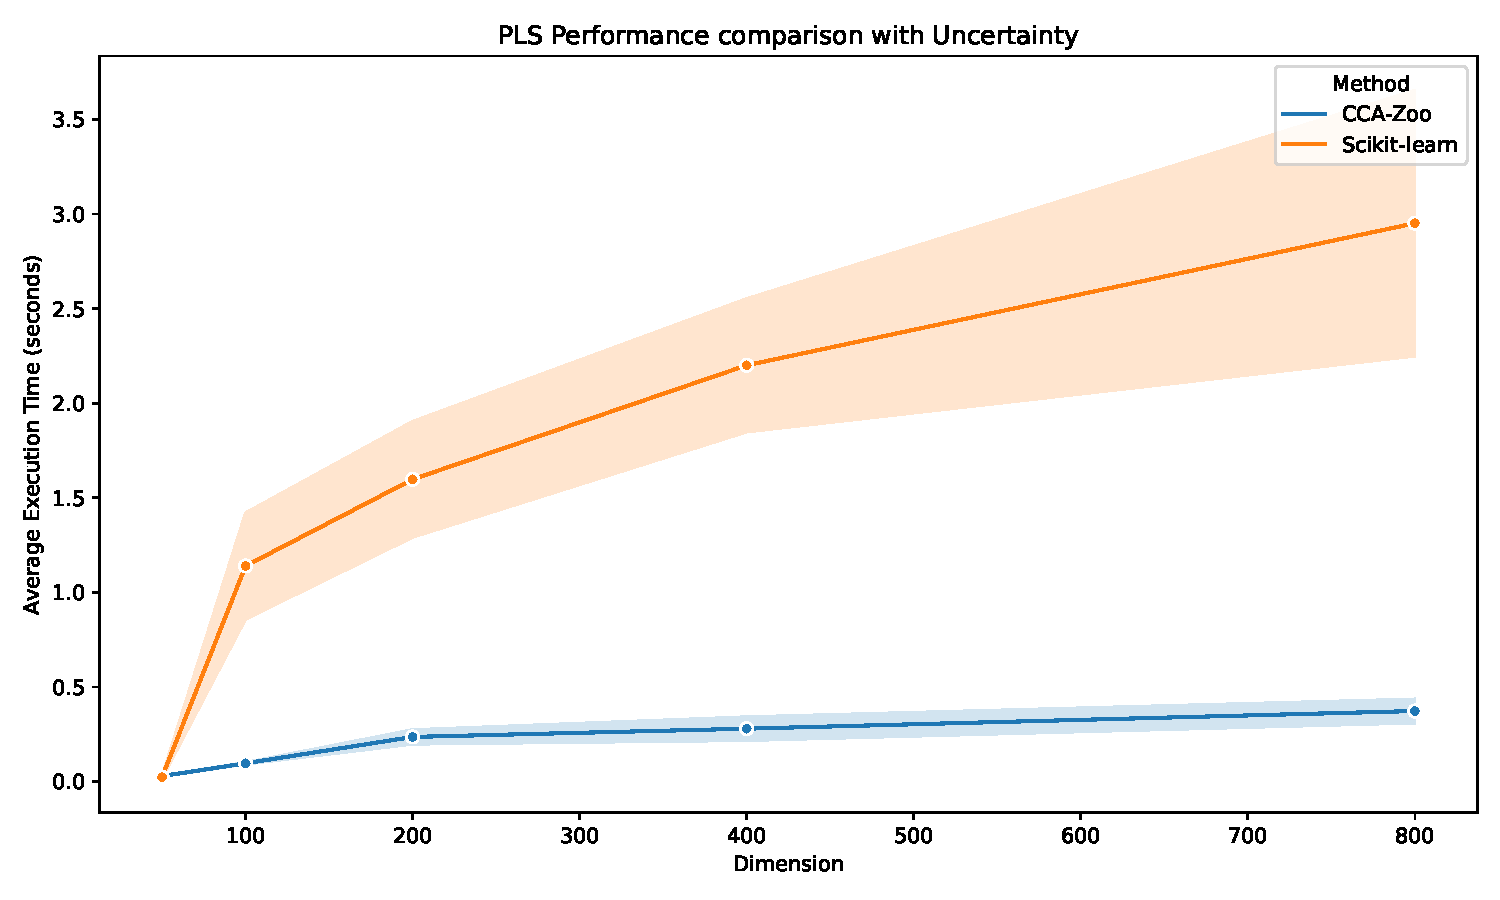
\includegraphics[width=0.9\textwidth]{figures/PLS_Speed_Benchmark}
    \caption{Performance comparison for PLS methods}
    \label{fig:pls_benchmark}
\end{figure}

The results indicate that \texttt{CCA-Zoo} is an efficient Python package for both CCA and PLS methods, holding its own against the widely-used \texttt{scikit-learn} library.
These experiments underscore the capability of \texttt{CCA-Zoo} to handle high-dimensional data efficiently, making it a suitable choice for applications in bioinformatics, natural language processing, and other high-dimensional data domains.

\section{Discussion}

\texttt{CCA-Zoo} fills a big gap in Python's tools for multiview learning.
It makes many multiview learning methods easy to use for Python users.
This package works well with known Python libraries like \texttt{scikit-learn}, \texttt{PyTorch}, and others, making it user-friendly.

\texttt{CCA-Zoo} is as good as \texttt{scikit-learn} in speed, especially for big data tasks in CCA and PLS. This is important for fields like bioinformatics where data is often large.

The package offers various methods, like linear, deep, and probabilistic models, and includes many datasets and tools for picking models and showing results.
This makes \texttt{CCA-Zoo} flexible and useful for different tasks.

A key goal of this thesis was to create practical tools for researchers, and \texttt{CCA-Zoo} achieves this.
It includes most methods from the thesis, ready for use.
This should help more people use and develop multiview learning methods.

In conclusion, \texttt{CCA-Zoo} is a valuable addition to Python's machine learning tools.
It offers a wide range of multiview learning methods in an efficient, easy-to-use package.
